\chapter{Introduction}
\label{cha:intro}

\textit{A computer program is said to \textbf{learn} from experience E with respect to some class of tasks T and performance measure P, if its performance at task in T, as measured by P, improves with experience E.}\\

Machine learning is the study of computer algorithms that improve automatically through experience. The peculiarity of machine learning algorithms is their ability to learn without being explicitly programmed. Due to these characteristics, ML is considered a component of the wider artificial intelligence field.
The environments of machine learning techniques application are never ending. Nowadays hot topics include speech recognition, optical character recognition, computer vision, autonomous driving, game playing, recommender systems (e.g. Amazon's "suggested for you" sections) and so on.

\begin{figure}
    \centering
    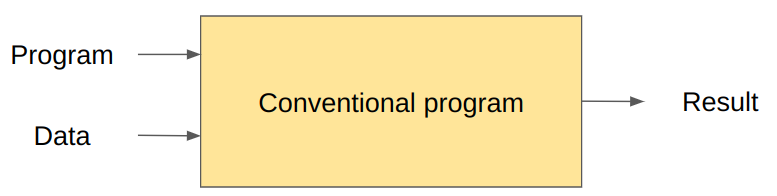
\includegraphics[width=\textwidth]{images/conventionalProgram.png}
    \caption{Conventional programming.}
    \label{fig:conventionalProgramming}
\end{figure}

\begin{figure}
    \centering
    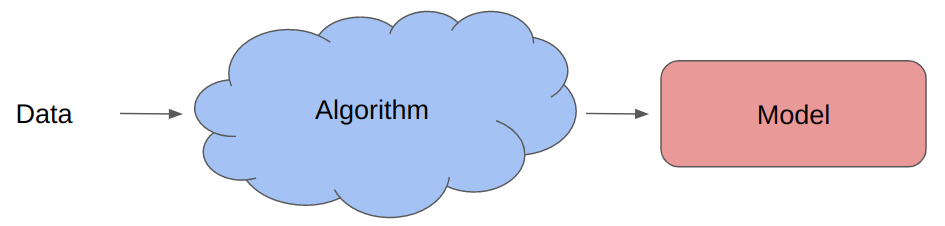
\includegraphics[width=\textwidth]{images/MachineLearningvsConventional.png}
    \caption{ML allows computers to \textbf{acquire knowledge}. Knowledge acquired is represented by a \textbf{model}. The model is used for \textbf{future} data.}
    \label{fig:mlvsconventionalProgramming}
\end{figure}

\subsubsection*{Components of a well-posted learning problem}
    A problem solvable through machine learning techniques relies on three well defined entities:
    \begin{itemize}
        \item the \textbf{task} that we are trying to solve (e.g. recognizing handwritten characters),
        \item a \textbf{performance measure} with which we will evaluate the performance of the algorithm (e.g. miss-classified items, scoring system...),
        \item the \textbf{training experience} on which the system relies on to learn (e.g. data with annotated solutions, labelled handwritten characters).
    \end{itemize}

\section{Design of a machine learning system}
    A proper design of a machine learning system follows six steps: 
    \begin{enumerate}
        \item formalize the learning task
        \item collect data
        \item extract features
        \item choose the class of learning models
        \item train the model
        \item evaluate the model
    \end{enumerate}
    
    \subsubsection*{Formalize the learning task}
        This is a overall definition of the goal we are trying to achieve. This could also be composed by a chain of separate tasks.\\ 
        Along the definition of the aim, it is required to define an appropriate performance measure for evaluating the system.\\
        With this first process, we get a formal definition of the problem. \newline
        \textbf{Example:} recognizing handwritten characters from images.
    
    \subsubsection*{Collect data}
        A machine learning system requires data, collected in machine readable format, on which the algorithm will rely for training. This is a delicate and difficult process because could imply manual intervention for labelling data.\\
        Not every machine learning technique requires annotation of data (semi-supervised and unsupervised learning).
        
    \subsubsection*{Extract features}
        The process of feature extraction consists in representing data in a way in which a computer can work with, this implies codifying data into other representative data.
        Prior knowledge is often needed in order to extract significant features. The number of features chosen has a relevant impact on the performances: too many features can require a number of training data much greater, too few could miss relevant information and decrease the performance. Moreover, by taking into account too many features, there is the risk of including noisy features which can make the learning problem harder.
    
    \subsubsection*{Choose the class of learning models}
        The choice of the model can heavily impact performance, a simple model classifier could be insufficient to complete the task while a complex model could lead to \textit{overfitting}. 
        % \defi{\textbf{Overfitting} \label{def:overfitting}\\ Overfitting is a modeling error that occurs when a function is too closely aligned to a limited set of data points. This happens when in training we achieve top performance while with validation sets they get lower: this could mean that the training took into account also noise among the training data.}
        \defi{\textbf{Overfitting}\label{def:overfitting}\\
        Overfitting is a modeling error that occurs when a function is too closely aligned to a limited set of data points. This happens when in training we achieve top performance while with validation sets they get lower: this could mean that the training took into account also noise among the training data.}
        
    \subsubsection*{Train the model}
        Training a model implies searching through the space of the possible models given a model class while performance of the model is measured. A trained model should be able to \textbf{generalize} (perform well on unseen data) and avoid overfitting \ref{def:overfitting}.
        Several techniques can be exploited to improve generalization.
        
    \subsubsection*{Evaluate the model}
        The evaluation of the model is based on data which the algorithm has never seen before. This process identifies weaknesses and give hints on how to improve the model. 
        Appropriate statistical test need to be carried on to verify significance of the observed results. 

\section{Learning settings}
    
    \subsection{Types of learning methods}
        \begin{figure}
            \centering
            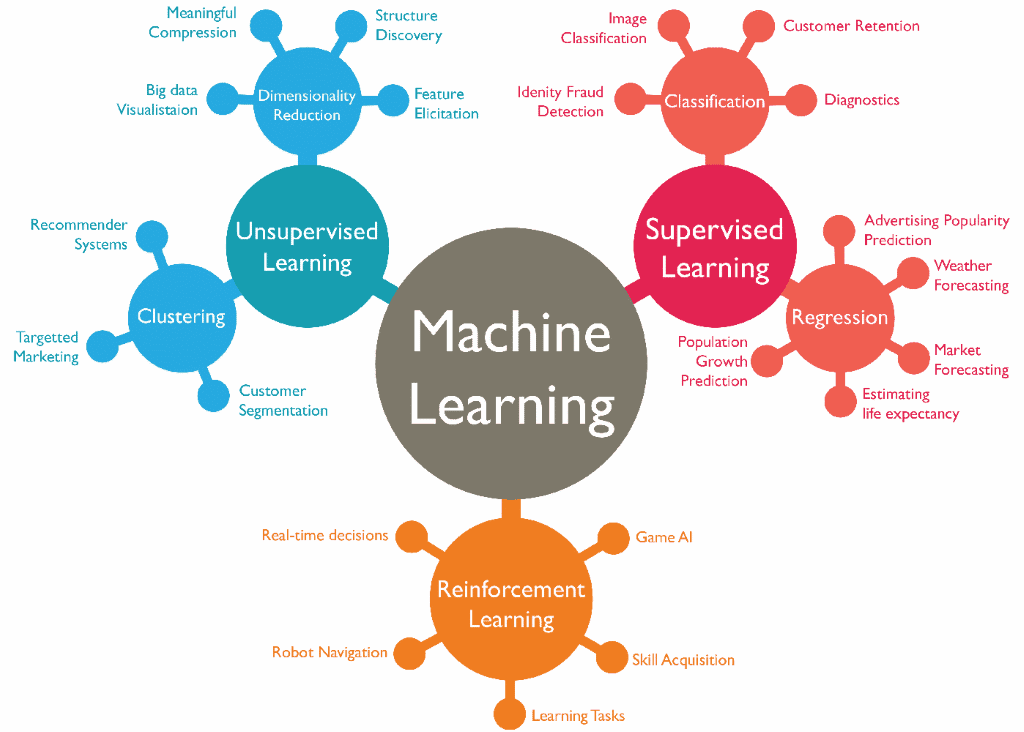
\includegraphics[width=\textwidth]{images/algoritmi-machine-learning.png}
            \caption{Main types of learning methods}
            \label{learning_methods_fig}
        \end{figure}
        
        Before starting to build a model, it is necessary to choose a type of learning. Often different data or goals require different learning settings.
        
        \defi{\textbf{Supervised learning \label{def:supervised}\\}
        The learner is provided with a set of input and output pairs (labelled data)
        $(x_i, y_i) \in \mathcal{X} \times \mathcal{Y}$.\\
        The learned model $f : \mathcal{X} \rightarrow \mathcal{Y}$ should map input samples into the proper output.
        A domain expert is often required in order to get labelled inputs.
        }
        
        \defi{\textbf{Unsupervised learning \label{def:unsupervised}\\}
        The learner is provided with a set of input but no annotation
        $(x_i)\in \mathcal{X}$.\\
        The learner models training example, e.g. by grouping them into clusters according to their similarity. These algorithms discover hidden patterns or data groupings without the need for human intervention.
        }
        
        \defi{\textbf{Semi-Supervised learning \label{def:semi-supervised}\\}
        The learner is provided with a set of input and output pairs (labelled data)
        $(x_i, y_i) \in \mathcal{X} \times \mathcal{Y}$ and a typical much bigger set of unlabelled data $(x_i)\in \mathcal{X}$.\\
        The learned model $f : \mathcal{X} \rightarrow \mathcal{Y}$ should map input samples into the proper output like in supervised learning while unlabelled data can be exploited to improve performances (e.g. improve boundaries).
        }
        
        \defi{\textbf{Reinforcement learning \label{def:reinforcement}\\}
        The learner is provided with a set of possible states $\mathcal{S}$ and for each of them a set of possible action $\mathcal{A}$ is available in order to move through the next state. 
        Performing an action $a$ from a state $s$ provides an immediate reward $r(s, a)$ that can be either immediate or delayed.\\
        The goal is learning a policy that allows the algorithm to choose between states maximizing the overall reward. Often the model needs to face exploitation (performing moves that are known to be rewarding) and exploration (perform new moves) to avoid getting stuck in a local minimum.
        }
    
    \subsection{Types of supervised learning tasks}
        Before starting to build a model, it is necessary to understand the goal. This implies understand what kind of classification we are trying to get once the problem is formalized.
        
        \defi{\textbf{Binary classification} \label{def:binary_classification}\\
        The binary classification problem sets its goal into separate samples into two subset (often defined as positive and negative).
        }
        
        \defi{\textbf{Multiclass classification} \label{def:multiclass_classification}\\
        The multiclass classification assigns a sample to a class chosen between $n>2$ different classes. 
        \begin{equation}
            f: \R^d \rightarrow \{1,2,\hdots, n\}
        \end{equation}
        
        }
        
        \defi{\textbf{Multilabel classification} \label{def:multilabel_classification}\\
        The multilabel classification assigns a sample to a subset of possible classes (not a unique assignment). E.g. predict the topics of a text.
        }
        
        \defi{\textbf{Regression} \label{def:regression}\\
        This type of problems require to assign a real value to a sample.
        \begin{equation}
            f: \R^d \rightarrow \R
        \end{equation}
        }
        
        \defi{\textbf{Ordinal regression or ranking} \label{def:ranking}\\
        A ranking problem sets its goal into defining an order to samples according to their relevance/quality/importance.
        }
        
    \subsection{Types of unsupervised learning tasks}
        
        \defi{\textbf{Dimensionality reduction} \label{def:dimension_reduction}\\
        In dimensionality reduction tasks we are trying to reduce the dimension of the data maintaining as much information as possible.
        }
        
        \defi{\textbf{Clustering} \label{def:clustering}\\
        For clustering we mean divide data into homologous groups according with some chosen similarity.
        }
        
        \defi{\textbf{Novelty detection} \label{def:novelty}\\
        Tasks in which we are trying to detect anomalies. It consists in studying the standard behaviour of the system in order to detect novelty or unusual events.
        }
        
        Probabilistic reasoning in presence of uncertainty is fundamental. Evaluating of performances related to different variables and estimate probabilities and relation between variables is often implied.
        
    \subsection{Types of learning algorithms}
        Based on the knowledge we have in the field of research, we adopt different strategies:
        \begin{itemize}
            \item \textbf{Bayesian decision theory}: when we are certain of the probability distribution of the data
            \item \textbf{Parameter estimation}: when we know the probability distribution but parameters need to be adjusted
            \item \textbf{Discriminative or generative methods}: when we have available training data but we do not know their distribution 
            \item \textbf{Unsupervised methods}: when there is lack of data and also their distribution is unknown.
        \end{itemize}
    
    \subsection{Discriminative and Generative Models}
    Machine learning models can be classified into two types of models: \textit{discriminative} and \textit{generative} models. These notions have not been explicitly covered during the course. However, it could be useful to briefly introduce the differences between the two in order to get a slightly better and more complete understanding of the following. In simple words, a discriminative model makes predictions on the unseen data based on conditional probability and can be used either for classification or regression problem statements ($P(y | x)$). On the contrary, a generative model focuses on the distribution of a dataset to return a probability for a given example ($P(x)$).
    
    \paragraph{}
    
    Discriminative models are not capable of generating new data points. Therefore, the ultimate objective of discriminative models is to separate one class from another (i.e. learn boundaries). Training discriminative classifiers involve estimating a function $f: X \rightarrow Y$, or probability $P(Y|X)$.
    \begin{itemize}
        \item Assume some functional form for the probability such as $P(Y|X)$.
        \item With the help of training data, we estimate the parameters of $P(Y|X)$.
    \end{itemize}
    
    Examples of discriminative models are:
    
    \begin{itemize}
        \item Support Vector Machine (SVMs)
        \item Traditional neural networks
        \item Nearest neighbor
        \item Decision Trees and Random Forest
    \end{itemize}
    
    \paragraph{}
    
    Generative models are considered as a class of statistical models that can generate new data instances. These models are mainly used in unsupervised machine learning.
    Generative Adversarial Networks (GANs) are an example of generative machine learning model.\\
    What is more, generative models are capable of finding the conditional probability $P(Y|X)$, just as the discriminative counterpart. They estimate the prior probability $P(Y)$ and likelihood probability $P(X|Y)$ with the help of the training data and uses the Bayes Theorem to calculate the posterior probability $P(Y|X)$.
    \begin{equation}
        P(Y|X) = \frac{P(Y) \cdot P(X|Y)}{P(X)}
    \end{equation}
    As a result, generative models can tackle a more complex task than analogous discriminative models.
    
    \paragraph{}
    
    In essence, discriminative models draw boundaries in the data space, while generative models try to model how data is placed throughout the space. A generative model focuses on explaining how the data was generated, while a discriminative model focuses on predicting the labels of the data.
    
    \begin{figure}
        \centering
        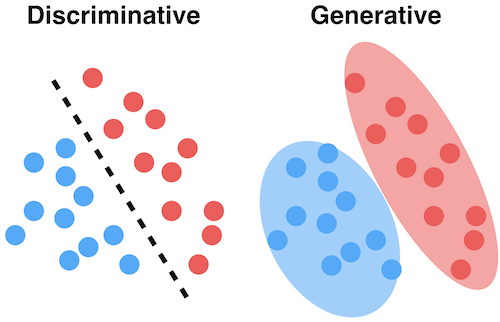
\includegraphics[width=0.5\textwidth]{images/descriminative_generative.png}
        \caption{Discriminative \textit{vs} Generative Models}
        \label{descriminative_generative}
    \end{figure}